\subsection{Desarrollo de la robótica a lo largo de la historia - Revisado por:A - Visto Bueno: A}

El mundo de la robótica da acceso a resolver una gran variedad de problemas donde el ser humano estaba
limitado físicamente: levantar cargas de gran peso, realizar tareas repetitivas durante tiempos
prolongados, etc. Además, como bien se sabe, ha permitido el desarrollo de cadenas de producción en
masa para poder desarrollar y crear los productos que usamos diariamente, desde el coche hasta el 
teléfono móvil.

Desde que se empezó a investigar en este campo, el desarrollo de los brazos robóticos ha sido 
exponencial: se empezó trabajando con pequeños autómatas hasta el desarrollo de la revolución
industrial \cite{moran_evolution_2007}.

Los primeros modelos, como se puede ver en la figura \ref{fig:evolution}, empezaron intentando hacer
representaciones de las manos humanas. En particular, se crearon un flautista y un tamborilero los
cuales eran capaces de tocar los respectivos instrumentos utilizando un complejo sistema de cables y 
engranajes para poder mover los ``dedos'' de los músicos.

\begin{figure}[H]
    \centering
    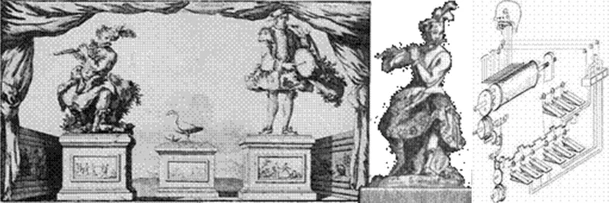
\includegraphics[width=.75\linewidth]{pictures/evolution_of_robotic_arms.png}
    \caption{flautista y tamborilero de Vaucanson \cite{vaucanson_mecanisme_1738}.}
    \label{fig:evolution}
\end{figure}

Siguiendo con esta idea, se fue mejorando y desarrollando el modelo de imitación de las articulaciones
y los miembros de los humanos, llegando a construir estructuras más complejas y avanzadas, pensadas en 
su momento para poder tocar el clavicordio mediante un muñeco, como se muestra en la figura 
\ref{fig:lady_musician}:

\begin{figure}[H]
    \centering
    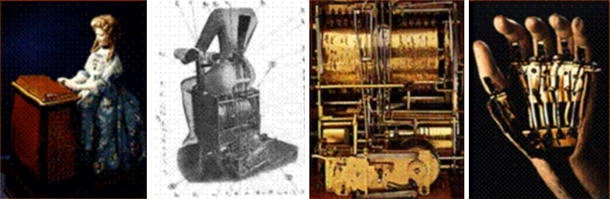
\includegraphics[width=.8\linewidth]{pictures/reproduction_of_lady_musician.png}
    \caption{en 1774, ``lady musician'' por Jaquet-Droz \cite{chapuis_alfred_and_droz_edmond_automata_1958}.}
    \label{fig:lady_musician}
\end{figure}

Durante los años siguientes, el proceso se fue refinando hasta el punto de desarrollar un autómata
el cual era capaz de jugar al ajedrez, llamado ``The Turk'' \cite{standage_tom_turk_2002}, construido
en 1769. La estructura comprendía un conjunto de mecanismos los cuales eran controlados por un operador,
encargado de realizar los movimientos del brazo izquierdo del autómata.

En la figura \ref{fig:turk} se puede ver cómo está diseñado el sistema para mover un controlador 
pantográfico sobre el tablero de juego, controlado por el operador externo antes mencionado:

\begin{figure}[H]
    \centering
    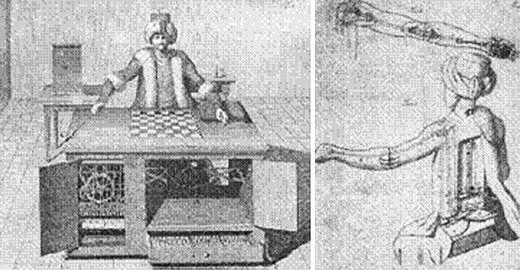
\includegraphics[width=.75\linewidth]{pictures/chess_evolution.png}
    \caption{``The Turk'', creado por von Kempelen en 1769 \cite{standage_tom_turk_2002}.}
    \label{fig:turk}
\end{figure}

Desde entonces, la robótica ha evolucionado y crecido de manera exponencial. Por una parte, debidas
las distintas guerras que han habido en los últimos 200 años, se ha dado un gran impulso a la 
industria encargada de crear distintos dispositivos con fines de defensa y ataque. En particular,
se potenciaron mucho los desarrollos de dispositivos por control remoto, destacando el diseño de
Nicola Tesla en 1898 de un barco completamente automatizado, controlado por control remoto y sumergible,
como se puede ver en la figura \ref{fig:nicola_tesla_boat}:

\begin{figure}[H]
    \centering
    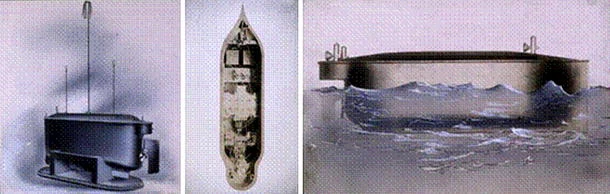
\includegraphics[width=.75\linewidth]{pictures/nicola_tesla_boat.png}
    \caption{barco a control remoto de Nicola Tesla, en 1898 \cite{belarmino_j_and_moran_me_and_firoozi_f_and_capello_s_and_kolios_e_and_perrotti_m_teslas_2005}.}
    \label{fig:nicola_tesla_boat}
\end{figure}

Por otro lado, dada la cantidad de bajas de las Primera y Segunda Guerras Mundiales, se empezaron a
desarrollar robots que permitieran sustituir a los militares en el campo de batalla, destacando en este
campo el robot ``Elektro'', creado por la compañía Westinghouse. Dicho robot supuso un gran éxito en la
industria de los robots y armamentística, pudiendo moverse completamente, disparar armas, mover elementos
faciales para ``expresar emociones'' e inclusive poder comunicarse.

En la figura \ref{fig:elektro}, se puede ver a la izquierda la primera versión ``Alpha'' y, a la derecha,
la versión mejorada ``Elektro'':

\begin{figure}[H]
    \centering
    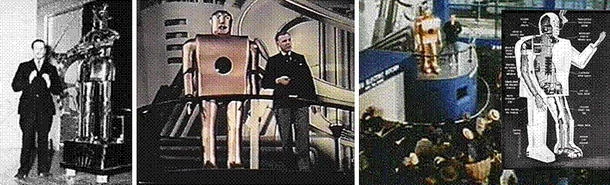
\includegraphics[width=.85\linewidth]{pictures/elektro.png}
    \caption{``Alpha'', el primer robot diseñado con fines militares y su posterior evolución, ``Elektro''.}
    \label{fig:elektro}
\end{figure}

Toda esta evolución ha acabado dando a la época actual, en donde tenemos robots sofisticados y con
distintos actuadores, pudiendo interactuar con muchísimos elementos de nuestro entorno y trabajar en
distintas fases de producción de cadenas de montaje en serie. Además, se trabaja continuamente para 
que cada vez los robots puedan realizar más tareas de los humanos, mejorando cada vez más los
``\textit{end--effectors}'' (controladores del final de los extremos del brazo). En la figura 
\ref{fig:new_robots} se puede ver cómo robots medianamente antiguos (del 2005) ya podían realizar diversas
actividades, como interactuar con las personas o tocar un instrumento.

\begin{figure}[H]
    \centering
    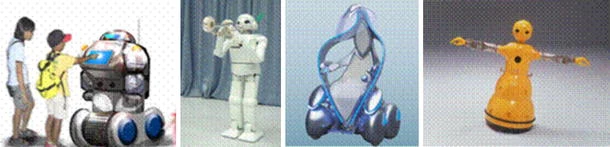
\includegraphics[width=.75\linewidth]{pictures/expo_japan.png}
    \caption{exposición mundial del 2005 en Japón \cite{belarmino_j_and_moran_me_and_firoozi_f_and_capello_s_and_kolios_e_and_perrotti_m_oriental_2005}.}
    \label{fig:new_robots}
\end{figure}

\subsection{Los brazos robóticos}

Con los avances actuales, el mundo de la robótica ha evolucionado a un nuevo nivel: con la inclusión
de los transistores en lugar de las válvulas de vacío se han podido desarrollar circuitos integrados
que manejan de manera mucho más sofisticada el control del brazo robótico.

En 1962, la empresa ``Unimate'' introdujo su primer brazo robótico de carácter industrial. Aproximadamente,
se vendieron 8500 unidades. Este hito es importante en tanto a que se valoraron por primera vez los
grados de libertad que debían de tener los brazos robóticos. 

Estos planteamientos derivaron en distintos robots famosos que incluso siguen en activo hoy día. En
1969, Victor Scheinman, de la Universidad de Standford, desarrolló un brazo robótico que funcionaba
alimentado por la electricidad y que se podía mover en los seis ejes, el cual se llamó ``el brazo de
Standford''. De forma paralela, Marvin Minsky, del MIT, desarrolló un brazo robótico para la investigación
naval, para exploración submarina. En particular, el brazo tenía veinte grados de libertad ya que el brazo
funcionaba mediante electricidad impulsando sistemas hidráulicos. Más tarde, Scheinman continuó
desarrollando brazos robóticos, creando el ``\textit{Programmable Universal Machine for Assembly}'',
más conocido como PUMA.

En la actualidad, los brazos robóticos se desarrollan y diseñan para seguir la estructura física
del cuerpo humano (ver figura \ref{fig:human_body}).

\begin{figure}[H]
    \centering
    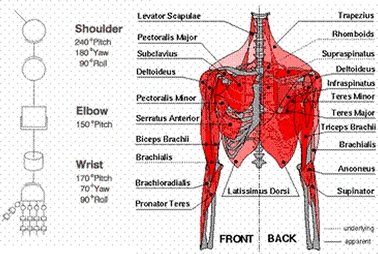
\includegraphics[width=.65\linewidth]{pictures/human_body.png}
    \caption{grados de libertad de un brazo robótico y estructura del cuerpo humano \cite{moran_evolution_2007}.}
    \label{fig:human_body}
\end{figure}

De esta estructura anterior, se deducen las siguientes partes:

\begin{itemize}
    \item Articulación del hombro: dispone de tres grados de libertad que permiten
    subir y bajar, ir a la izquierda y derecha, y rotar sobre sí mismo.
    \item Articulación del codo: el codo permite extender, contraer y reorientar tanto
    la muñeca como la mano. Por lo general, se estima la extensión del codo en unos
    150\textdegree.
    \item La muñeca: compone el último elemento del brazo robótico antes de llegar
    al ``\textit{end--effector}''. Es de los elementos más importantes debido a su
    gran capacidad de movimiento en las tres dimensiones. Sin esta articulación,
    el brazo robótico se asemejaría en funcionalidad a un robot pantográfico. Cada vez más,
    las articulaciones de la muñeca se vuelven complejas y sofisticadas. La muñeca humana,
    por ejemplo, puede moverse 45\textdegree desde el centro, pero se reduce mucho la
    capacidad de rotación de la misma. En la actualidad se está investigando cómo poder
    mejorar la relación de movimientos para permitir una mayor movilidad, pero las 
    singularidades siguen siendo un gran problema. Por ejemplo, el robot quirúrgico
    da Vinci, pese a lo avanzado que pueda parecer, tiene problemas de bloqueo de las muñecas
    del mismo cuando se acerca a posiciones singulares.
    \item La mano: supone un ``\textit{end--effector}'' diferenciado que define el propóstio
    y la capacidad del brazo robótico. La mano es una herramienta capaz de realizar múltiples
    acciones muy variadas entre sí. Actualmente, se sigue investigando de forma activa sobre
    ello para intentar implementar controles sensoriales, de presión y de movimiento en los
    ``\textit{end--effector}'' de los robots.
\end{itemize}

\subsection{La actualidad}
